% USEFUL LINKS:
% -------------
%
% - UiO LaTeX guides:          https://www.mn.uio.no/ifi/tjenester/it/hjelp/latex/
% - Mathematics:               https://en.wikibooks.org/wiki/LaTeX/Mathematics
% - Physics:                   https://ctan.uib.no/macros/latex/contrib/physics/physics.pdf
% - Basics of Tikz:            https://en.wikibooks.org/wiki/LaTeX/PGF/Tikz
% - All the colors!            https://en.wikibooks.org/wiki/LaTeX/Colors
% - How to make tables:        https://en.wikibooks.org/wiki/LaTeX/Tables
% - Code listing styles:       https://en.wikibooks.org/wiki/LaTeX/Source_Code_Listings
% - \includegraphics           https://en.wikibooks.org/wiki/LaTeX/Importing_Graphics
% - Learn more about figures:  https://en.wikibooks.org/wiki/LaTeX/Floats,_Figures_and_Captions
% - Automagic bibliography:    https://en.wikibooks.org/wiki/LaTeX/Bibliography_Management  (this one is kinda difficult the first time)
%
%                              (This document is of class "revtex4-1", the REVTeX Guide explains how the class works)
%   REVTeX Guide:              http://www.physics.csbsju.edu/370/papers/Journal_Style_Manuals/auguide4-1.pdf
%
%
% COMPILING THE .pdf FILE IN THE LINUX TERMINAL
% ---------------------------------------------
%
% [terminal]$ pdflatex report_example.tex
%
% Run the command twice, always.
%
% When using references, footnotes, etc. you should run the following chain of commands:
%
% [terminal]$ pdflatex report_example.tex
% [terminal]$ bibtex report_example
% [terminal]$ pdflatex report_example.tex
% [terminal]$ pdflatex report_example.tex
%
% This series of commands can of course be gathered into a single-line command:
% [terminal]$ pdflatex report_example.tex && bibtex report_example.aux && pdflatex report_example.tex && pdflatex report_example.tex
%
% ----------------------------------------------------



% \documentclass[english,notitlepage,reprint,nofootinbib]{revtex4-2}  % defines the basic parameters of the document
\documentclass[english,notitlepage,reprint,nofootinbib]{revtex4-2}  % defines the basic parameters of the document
% If you want a single-column, remove "reprint"

% Allows special characters (including æøå)
\usepackage[utf8]{inputenc}
% \usepackage[english]{babel}

% Note that you may need to download some of these packages manually, it depends on your setup.
% It may be usefult to download TeXMaker, because it includes a large library of the most common packages.

\usepackage{physics,amssymb}  % mathematical symbols (physics imports amsmath)
\include{amsmath}
\usepackage{graphicx}         % include graphics such as plots
\usepackage{xcolor}           % set colors
\usepackage{hyperref}         % automagic cross-referencing
\usepackage{listings}         % display code
\usepackage{subfigure}        % imports a lot of cool and useful figure commands
% \usepackage{float}
%\usepackage[section]{placeins}
\usepackage{algorithm}
\usepackage[noend]{algpseudocode}
\usepackage{subfigure}
\usepackage{tikz}
\usetikzlibrary{quantikz}
% defines the color of hyperref objects
% Blending two colors:  blue!80!black  =  80% blue and 20% black
\hypersetup{ % this is just my personal choice, feel free to change things
    colorlinks,
    linkcolor={red!50!black},
    citecolor={blue!50!black},
    urlcolor={blue!80!black}}


% ===========================================


\begin{document}

\title{FYS4150 - Project 2\\[0.5em]
  \small \href{https://github.com/isakrukan/FYS4150/tree/main/Project2}{\texttt{github.com/isakrukan/FYS4150/Project2}}
}
\author{Isak Cecil Onsager Rukan and Magnus Axelsen} % self-explanatory
\date{\today}                             % self-explanatory
\noaffiliation                            % ignore this, but keep it.
\maketitle

\section{Problem 1}
Consider a time-dependent horizontal beam of length \(L\) and \(u(x)\) the displacement of the beam at position \(x\in[0,L]\). A force is applied at \(x=L\) directed towards \(x=0\). The beam is fastened, and so \(u(0)=u(L)=0\), but is allowed to rotate: \(u'(x)\neq 0\).

This situation can be described by the second-order differential equation
\begin{align}
    \gamma \frac{d^2u(x)}{dx^2} = -Fu(x),
\end{align}
where \(\gamma\) is some constant. Introducing \(\hat{x}=x/L\) means that \(d\hat{x}^2 = dx^2/L^2\), and thus 
\begin{align}
    \frac{d^2u(\hat{x})}{d\hat{x}^2} 
    % = -\frac{L^2}{\gamma}Fu(\hat{x})
    = -\lambda u(\hat{x}),
\end{align}
where we have defined \(\lambda = FL^2/\gamma\).

\section{Problem 2}
In \texttt{src/triDag.cpp} a tridiagonal matrix is implemented as a class that provides a method \texttt{compute\_eigenvalues} which computes the eigenvalues and eigenvectors of the matrix. In \texttt{tests/test.cpp}, we run \texttt{test\_TriDag}, which tests that the correct eigenvalues and eigenvectors are computed for a tridiagonal matrix of size \(N=6\).

\section{Problem 3}
In \texttt{src/utils.cpp} we have created a function called \texttt{max\_offdiag\_symmetric}, which takes in a matrix \(A\) and two integers, \(k\) and \(l\). This function assumes that \(A\) is a symmetric matrix, and returns the greatest off-diagonal element of \(A\) (in absolute value) and updates \(k\) and \(l\) by reference to be the row and column indices of this element, respectively. We test that this is implemented correctly using 
\begin{align}
    A = \begin{pmatrix}
        1 & 0 & 0 & 0.5 \\ 
        0 & 1 & -0.7 & 0 \\ 
        0 & -0.7 & 1 & 0 \\ 
        0.5 & 0 & 0 & 1,
    \end{pmatrix}
\end{align} 
for which \texttt{max\_offdiag\_symmetric} should return \(-0.7\) and set \((k,l)=(2,1)\).


\section{Problem 4}
\subsection*{a)}
The Jacobi algorithm is implemented in \texttt{src/jacobi\_eigensolver.cpp}.
The program is broken down into a function \texttt{jacobi\_rotate()} performing one single Jacobi rotation, and a function \texttt{jacobi\_eigensolver()} repeatedly calling \texttt{jacobi\_rotate()} until the matrix is diagonal within some tolerance. 

\subsection*{b)}
A test function \texttt{test\_jacobi()} is implemented in \texttt{tests/test.cpp}.
The function constructs a $6\times6$ tridiagonal matrix and compares the eigenvalues and eigenvectors computed by the Jacobi algorithm to the analytic solutions.


\section{Problem 5}
\subsection*{a)}
We apply the Jacobi algorithm for different matrix sizes \(N\), and count the number of transformations required for the algorithm to converge.
Assuming the the number of required iterations roughly follows a power law \(O(N^k)\), one can estimate the exponent \(k\) by linear regression on a log-log scale.
The results are shown in figure \ref{fig:iterations}, and we find that \(k\approx 2.06\).
\newline
\newline
\subsection*{b)}
Whereas a tridiagonal matrix starts with \(O(N)\) off-diagonal elements, the corresponding number for a dense matrix will be \(O(N^2)\).
Given that the tridiagonal case scales roughly as \(O(N^2)\), one may therefore expect that the additional factor of \(N\) in the number of off-diagonal elements leads to an additional factor of \(N\) in the number of required transformations.
That is, one expects the dense case to scale as \(O(N^3)\).

\begin{figure}
    \centering
    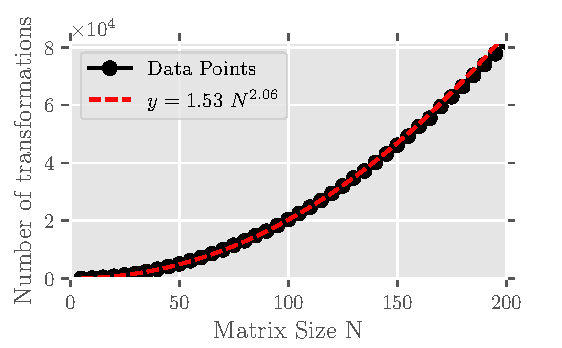
\includegraphics{Code/output/iterations.pdf}
    \caption{Number of transformations required for the Jacobi algorithm to converge for different matrix sizes \(N\).}
    \label{fig:iterations}
\end{figure}

\section{Problem 6}
The three lowest eigenmodes of the beam, for different numbers of discretization steps, are shown in figure \ref{fig:eigenvectors}. 
The analytic solutions are also included for comparison.
Notably, the numerical solutions are quite accurate even when the number of discretization steps is relatively small.
\begin{figure}
    \centering
    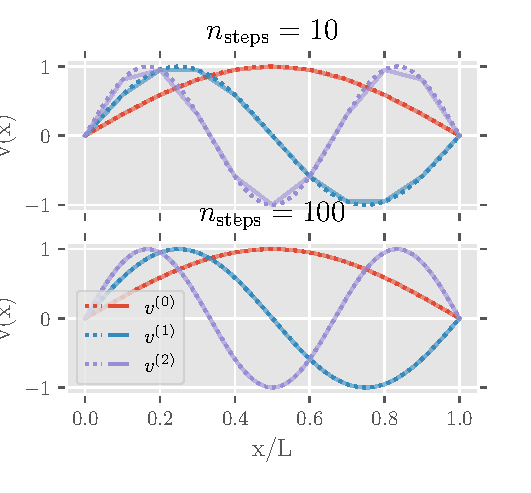
\includegraphics{Code/output/eigenvectors.pdf}
    \caption{The three lowest eigenmodes of the beam, for different numbers of discretization steps.
    Numerical solutions are given by the solid lines, with corresponding analytic solutions given by the dashed lines.}
    \label{fig:eigenvectors}
\end{figure}

\section{Code Implementation}
Details of the code implementation can be found in \href{https://github.com/isakrukan/FYS4150/blob/main/Project2/docs/doc.pdf}{doc.pdf.} (This is perhaps not exactly what this project needs, when it comes to code documentation that is. However, we have spent some time learning how to use \href{https://www.doxygen.nl/}{doxygen}, which creates \href{https://github.com/isakrukan/FYS4150/blob/main/Project2/docs/doc.pdf}{doc.pdf}, with the hopes that this can be beneficial in the upcoming projects.)



\onecolumngrid
% \bibliographystyle{apalike}
\bibliographystyle{unsrt}
\bibliography{ref}


\end{document}